\chapter{High-Order PRDC}
本章では,圧縮後のファイルから特徴抽出を行う手法であるPRDCに着目する.
そして,圧縮後のファイルから別の特徴を新たに抽出することでPRDCを改良する.

まず,PRDCが使用する圧縮率は,テキスト内の単語頻度のみで決定され
異なる単語間の関係を一切利用していない特徴であることを指摘する.そして,隣接
する単語関係を表す新しい特徴量を提案する.その後で新しい特徴量をPRDCに組み込んだ
手法を提案する.

\section{圧縮率} % (fold)
\label{sec:圧縮率}
PRDCが利用する圧縮率について考察する.PRDCではLZWアルゴリズムを用いて,基底辞書$D$に単語とそれに対応する符号(出力記号)
のペアを登録する.符号の長さは元の単語長よりも小さい.そして,圧縮時には入力テキスト$T$を前方からスキャンし,
$T$内の単語を対応する符号に順次置き換えることで圧縮を実現する.
一般に$T$を辞書$D$を使って圧縮した時の圧縮率は
\begin{eqnarray}
圧縮率 &=& \frac{圧縮後のファイルサイズ}{元テキストTのサイズ} \nonumber \\
&=& \frac{圧縮後の符号数 * 1符号の\mbox{bit}長}{Tの文字数 * 1文字の\mbox{bit}長} \nonumber \\
&=& \frac{圧縮後の符号数}{Tの文字数} * \alpha
%&= \frac{\sum_{i=1}^n m_i}{元のテキストの長さ} * \alpha
\label{eq:compress}
\end{eqnarray}
と記述できる.だたし,$\alpha=\frac{1符号の\mbox{bit}長}{1文字の\mbox{bit}長}$を表す定数である.

ここで辞書$D$に$n$種類の単語$(w_1,w_2,..,w_n)$が登録されているとする.単語$w_i$の文字数を$l_i$とおく.
さらに$T$内の単語$w_i$の出現回数を$m_i$と記述する.この時,式(\ref{eq:compress})における
圧縮後の符号数は$\sum_{i=1}^n m_i$である.一方,$T$の長さは$\sum_{i=1}^n m_il_i$になる.
従って,式(\ref{eq:compress})は次のように書き換えられる.
\begin{equation}
\begin{split}
圧縮率 &= \frac{\sum_{i=1}^n m_i}{\sum_{i=1}^n m_i l_i} * \alpha \cr
&= 1-(1-\frac{\sum_{i=1}^n m_i}{\sum_{i=1}^n m_i l_i}) * \alpha \cr
&= 1- \frac{\sum_{i=1}^n m_i(l_i -1)}{\sum_{i=1}^n m_i l_i} * \alpha \cr
&= 1- \frac{\sum_{i=1}^n m_i(l_i -1)}{Tの長さ} * \alpha
\end{split}
\label{eq:ncomp}
\end{equation}
$l_i -1$は$w_i$の符号化1回で削減される文字数であり,$m_i(l_i -1)$は,$w_i$の符号化に
より元のテキストから何文字削減できるかを表す.
式(\ref{eq:ncomp})が示すように圧縮率は各単語の出現頻度のみで決定される特徴量であり,
$T$内における異なる単語の関係は考慮しない.例えば,どの単語とどの単語が$T$内で
隣接して出現するかという情報は圧縮率には反映されない.
%元テキストにおける単語の隣接関係は全く考慮されていない.
% section 圧縮率 (end)

\section{単語の隣接関係を抽出する単純な手法} % (fold)
\label{sec:単語の隣接関係を抽出する単純な手法}
前節で述べたように,基底辞書による圧縮率は$T$に各単語が何回含まれるかによって決定される特徴量であるが,これは$T$内でどの単語が隣接して出現するかという情報を捨ててしまっている.
隣接関係を抽出する単純な方法としては,図~\ref{fig:image/N-Gram.eps}のように,元のオブジェクト列をN-Gramのようにグループ分けし,そのヒストグラムから特徴を抽出する事が考えられる.しかし,この手法ではいくつの符号を1グループにするかという追加のパラメータが必要になり,PRDCを手軽さの面で下回る.

\begin{figure}[tb]
\begin{center}
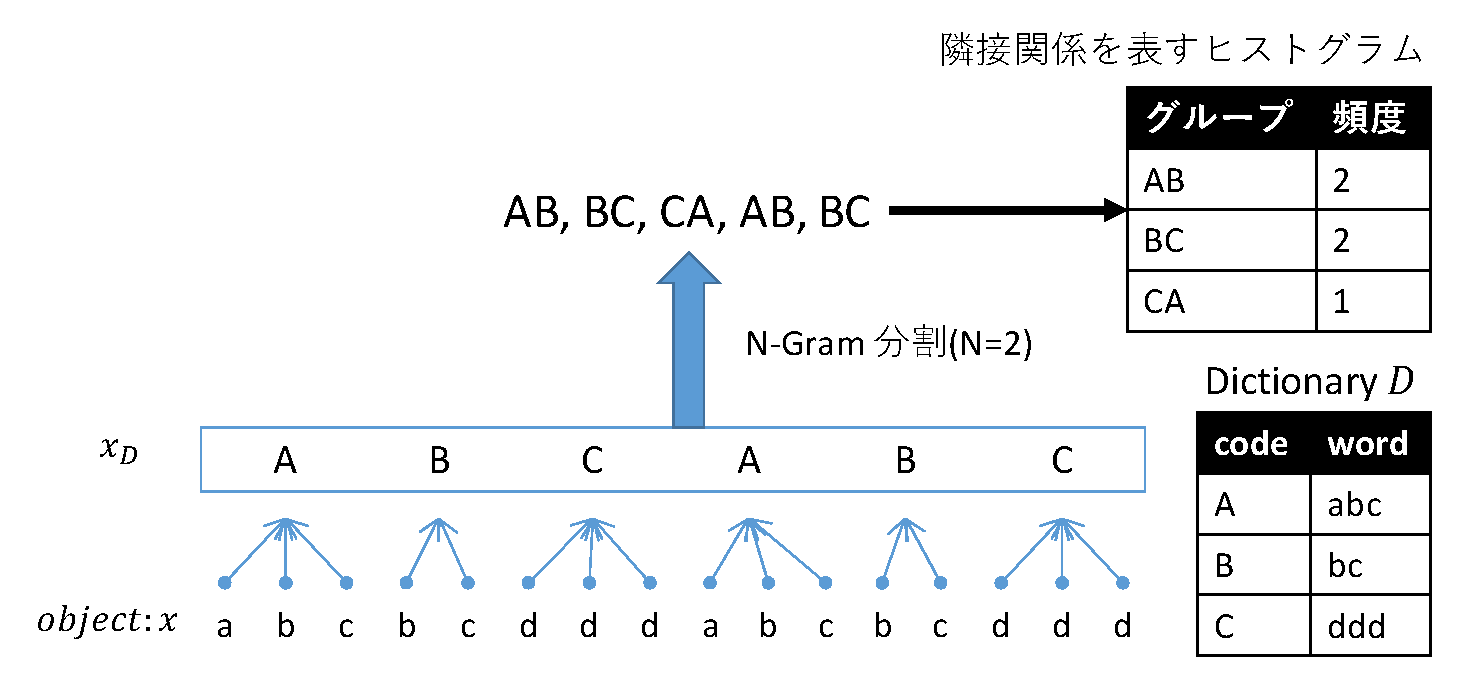
\includegraphics[clip, width=\columnwidth]{image/N-Gram.eps}
\caption{符号列からN-Gramのヒストグラムを作成}
\label{fig:image/N-Gram.eps}
\end{center}
\end{figure}


% section 単語の隣接関係を抽出する単純な手法 (end)

\section{再圧縮による単語の隣接関係の抽出}
\begin{figure}[tb]
\begin{center}
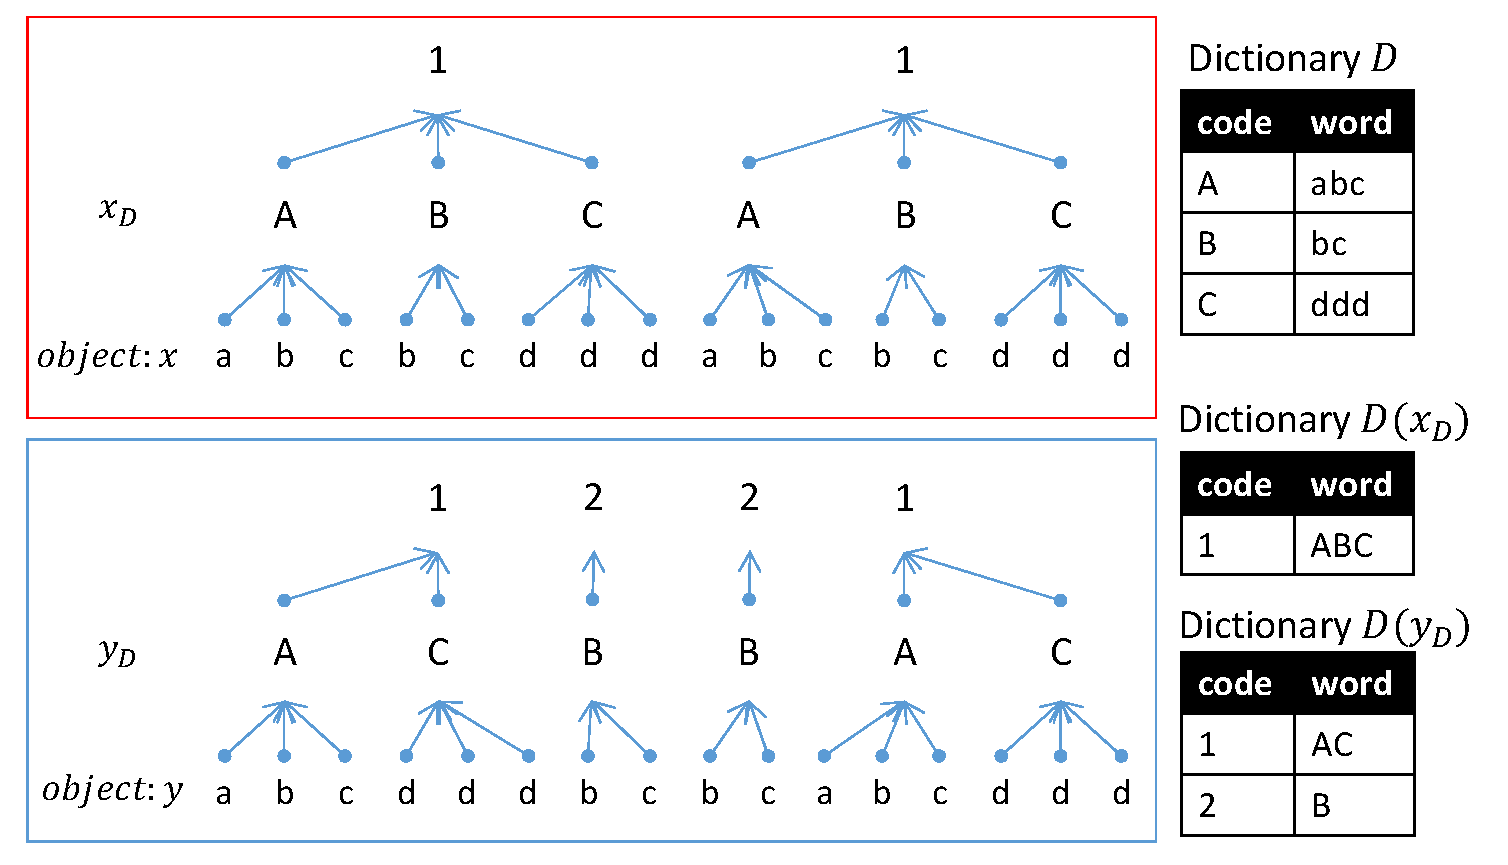
\includegraphics[clip, width=\columnwidth]{image/recompress.eps}
\caption{圧縮後のファイルの再圧縮}
\label{fig:image/recompress.eps}
\end{center}
\end{figure}

本研究では$T$内での単語の隣接関係から定まる新しい特徴量を圧縮後のファイルから抽出する.
具体的には,$T$を辞書$D$で圧縮後のファイル(符号列)を$A^T_D$とすると,$A^T_D$をもう一度再圧縮を行った時の圧縮率を特徴量として採用する.
$A^T_D$の再圧縮では,辞書$D$で圧縮するのではなく,$A^T_D$から構築した辞書で$A^T_D$自身を圧縮する.すなわち,$A^T_D$の自己圧縮率を再圧縮率とする.
再圧縮率の詳しい求め方をAlgorithm\ref{algo:recompress}に示す.
\begin{algorithm}[tb]
\caption{再圧縮率の算出}\label{algo:recompress}
\begin{algorithmic}[1]
\Procedure{CalcRecompressRate}{$A^T_D$}
\Comment{$A^T_D$は1度目の圧縮で出力された符号列}
\State{$Dictionary = 空の辞書$}
\State{$OutputLength = 0$}\Comment{出力長}
\State{$index = 0$}\Comment{辞書番号}
\State{$w = \{\}$}
\For{$i = 1 \, \ldots \, A^T_D.\mathrm{length}$}
\State{$c = A^T_D[i]$}
\State{$wc = w + \{c\}$}\Comment{符号列$w$と符号列$\{c\}$を連結}
\If{$符号列cが辞書に存在しない$}
\State{$Dictionary[\{c\}] = index$}\Comment{初めて出現した符号列$c$を辞書に登録}
\State{$index++$}
\EndIf
\If{$符号列wcが辞書に存在する$}
\State{$w = wc$}
\Else
\State{$Dictionary[wc] = index$}\Comment{符号列$wc$を辞書に登録}
\State{$index++$}
\State{$OutputLength++$}
\State{$w = \{c\}$}
\EndIf
\EndFor
\If{$wが空でない$}
\State{$OutputLength++$}
\EndIf
\State{$RecompressRate = OutputLength / A^T_D.\mathrm{length}$}
\State \textbf{return} $RecompressRate$
\EndProcedure
\end{algorithmic}
\end{algorithm}


再圧縮率が$T$内の単語の隣接関係から定まる特徴であることを例によって示す.
%一度目の圧縮率だけでは分類できないオブジェクトを分類する.
図\ref{fig:image/recompress.eps}は,テキスト$T_1$と$T_2$を再圧縮まで行った時の様子を示す.
最下段が元のテキストであり,真ん中の段が辞書$D$で圧縮後のファイル,最上段が再圧縮後の出力ファイルである.
なお,再圧縮時には自己圧縮を行うため,$T_1$の再圧縮と$T_2$の再圧縮では異なる辞書が用いられている.

辞書$D$で$T_1,T_2$を圧縮後の符号化列はそれぞれ''ABCABC'',''ACBBAC''と異なっている.しかし,圧縮率は
どちらも$\frac{6}{16}=0.375$となって$T_1$と$T_2$は区別できない.これは符号語'A','B','C'の出現回数
が同じであることが理由であり,3.1節で述べたように単語の出現回数のみで決定される圧縮率の限界である.

一方,$T_1$の再圧縮率は$\frac{2}{6}$,$T_2$の再圧縮率は$\frac{4}{6}$と異なる値になり,$T_1$と$T_2$を
区別できる.この違いは$T_1$と$T_2$の単語順序の違いに起因する.例えば,$T_1$の再圧縮率は符号語列
'ABC'が$T_1$内に2回出現した事実を反映する.このように再圧縮率は単語の隣接関係から定まる特徴である.

%xとyの区別がつかない.もう一度圧縮を行うことで,符号列の構造を表した特徴量を抽出する事ができる.
\section{再圧縮率を利用したPRDC}
%\section{圧縮率ベクトル} % (fold)
本節では,前節で提案した再圧縮率をPRDCに組み込んだ手法を提案する.
従来のPRDCでは,テキスト$x$を$N$個の基底辞書集合$\{D_1,D_2,\dots,D_N\}$で圧縮し,その圧縮率を並べた$N$
次元特徴ベクトル(式(\ref{eq:PRDC}))で$x$を表現する.
一方,提案手法では通常の圧縮率と再圧縮率を合わせた特徴ベクトルを構築する(図\ref{fig:HOPRDC.eps}).

\begin{figure}[tb]
\centering
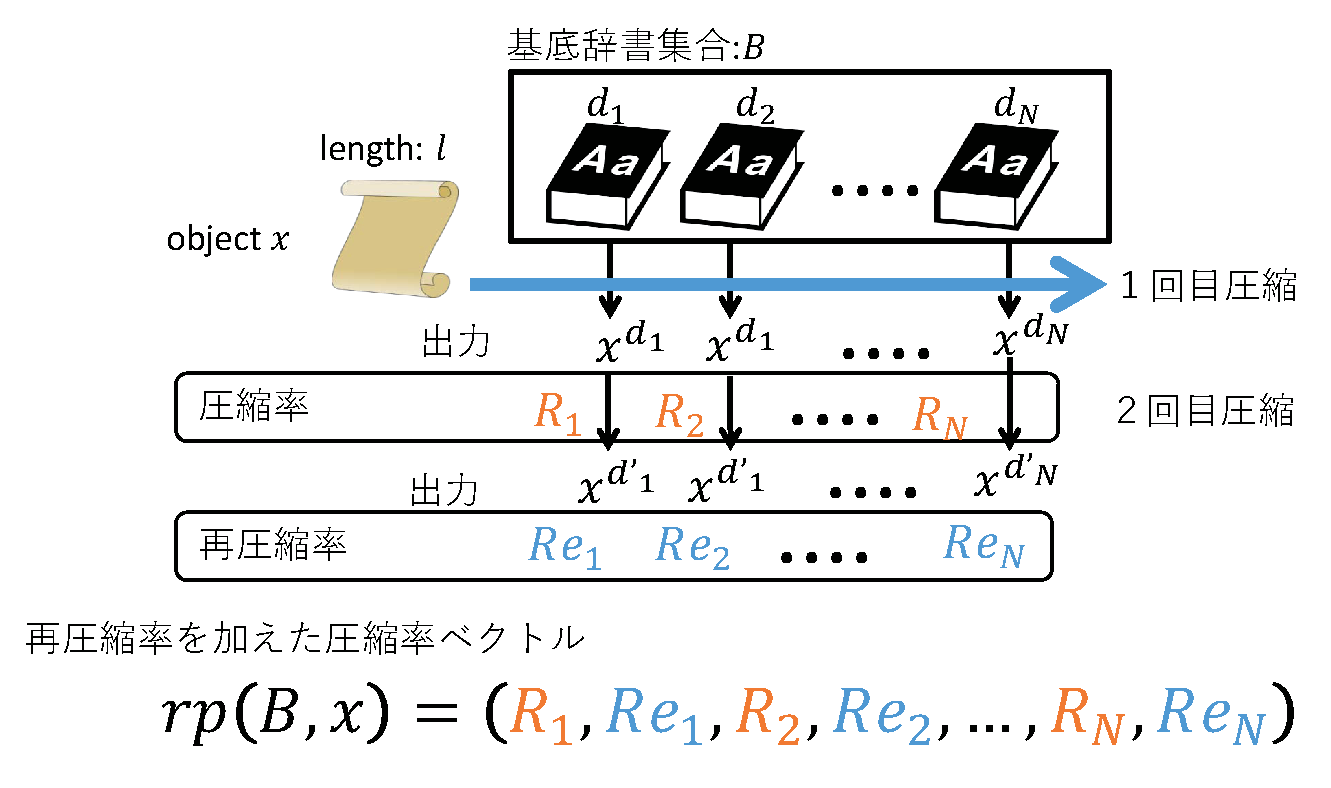
\includegraphics[clip, width=\columnwidth]{image/HOPRDC.eps}
\caption{再圧縮率を加えた圧縮率ベクトルの作成}
\label{fig:HOPRDC.eps}
\end{figure}

基底辞書集合$\{D_1,D_2,\dots,D_N\}$を用いた,オブジェクト$x$に対する再圧縮率を加えた圧縮率ベクトルは
$\boldsymbol{rp}(B,x)$は次のように定義される.
\begin{equation}
\boldsymbol{rp}(B,x) = \biggl(\frac{l'_1}{l}, \frac{l''_1}{l_1'}, \frac{l'_2}{l}, \frac{l''_2}{l'_2}, \dots, \frac{l'_N}{l}, \frac{l''_N}{l'_N} \biggr)
\end{equation}
\begin{itemize}
	\item $l $:入力オブジェクト長
	\item $l'_i$: $x$を$D_i$で圧縮したときの出力長
	\item $l''_i$: $x$を$D_i$で圧縮した符号列を,再圧縮したときの出力長
\end{itemize}
である.1つの基底辞書が2つの次元に対応するので,圧縮率ベクトルの次元数は$2N$になる.この圧縮率ベクトルは
以下の特徴を有する.
\begin{enumerate}
	\item 通常の圧縮率により単語の頻度を考慮する.
	\item 再圧縮率により単語の隣接関係を考慮する.
\end{enumerate}
提案手法では単語の頻度だけでなく単語の隣接関係まで考慮したパターン認識を可能にする.
この性質より,提案手法をHOPRDC (High-Order PRDC, 高階PRDC)と名付ける.

HOPRDCはPRDCと比べて追加のハイパパラメータを必要としておらず,利用の手軽さを失っていない.

%\label{sub:再圧縮率を取り入れたprdc}
\chapter{Weigtbed NMD} % (fold)
本章では,圧縮辞書から特徴抽出を行う手法であるNMDを取り上げ,
圧縮辞書からの新しい特徴抽出によるNMDの改良手法を説明する.
\label{sec:nmdの改良_仮_}
\section{NMDの課題}
NDDやNMDなどの辞書間距離では,辞書を元オブジェクトの要約として用いることで,類似度計算の計算量を削減する.
その一方で,元オブジェクトから情報を捨てることが欠点である.NMDでは各単語の出現回数を考慮し,NDDよりも捨てられる情報を削減した.
しかし,NMDでは辞書に登録された単語長を無視し,全単語は長さによらず均等の重みを持つものとして式(\ref{eq:NMD})の定義
に従って距離計算を実施する.つまり,単語が元のオブジェクトで占めている割合を考慮していない.

図~\ref{fig:image/NMD_Task.eps}は,NMDで使用する多重集合中の単語の割合と,元オブジェクトにおける単語の割合の一例である.オブジェクト$x$は全体で7文字なので,3文字の単語"aaa"がオブジェクト$x$中で占める割合は3/7である.対して,単語"aaa"が多重集合$MS(x)$中で占める割合は,"aaa"の重複度が1なので1/4となる.
このように,NMDのように全単語を均等に取り扱う手法では,元オブジェクトにおいて単語が占める領域の割合と,
各単語が類似度計算に与える影響の割合が乖離する.

\begin{figure}[tb]
\begin{center}
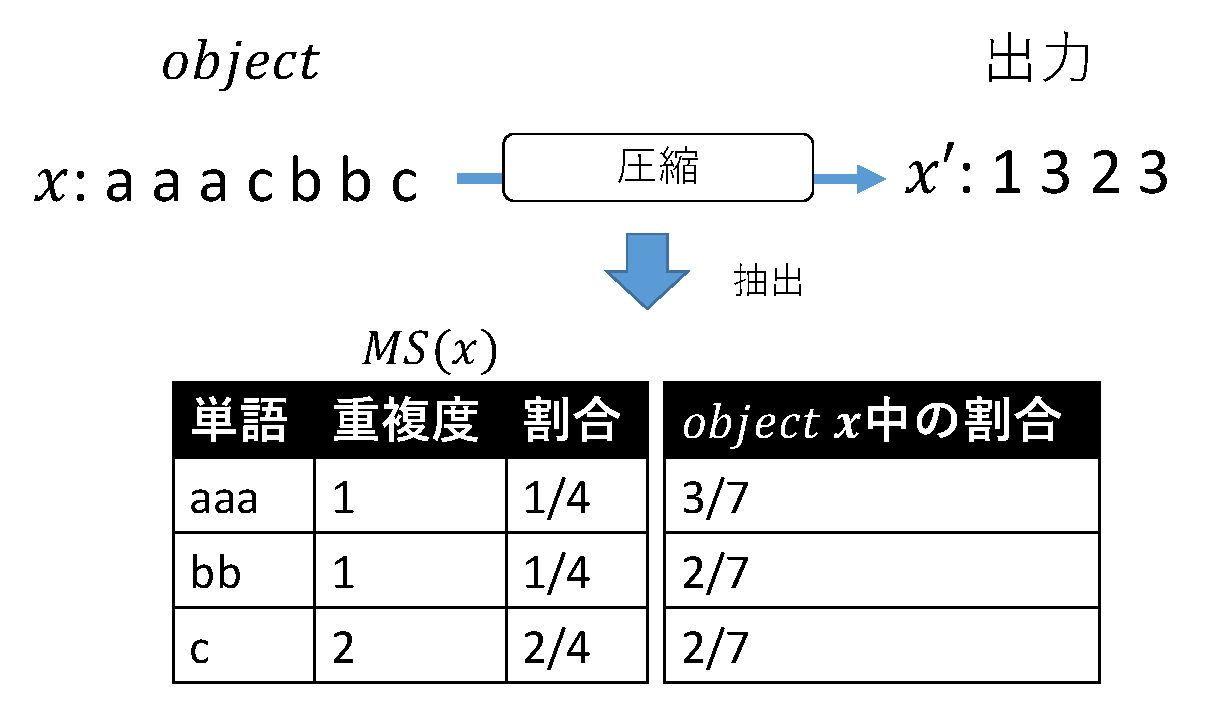
\includegraphics[clip, width=\columnwidth]{image/NMD_Task.eps}
\caption{単語の多重集合中の割合とオブジェクト中の割合}
\label{fig:image/NMD_Task.eps}
\end{center}
\end{figure}

距離計算の際,単語長を無視することがパターン認識に与える影響を考えてみよう.図\ref{fig:created_image.eps}左の画像は,
上半分が単純な領域で,下半分が複雑な領域になっている.このような画像の現実例としては上半分が海で下半分が港湾都市
であるケースが挙げられる.この画像から辞書を作ると,上領域からは長い単語が少数生成され,下領域からは
短い単語が多数生成される(図\ref{fig:created_image.eps}右).この時,全単語を均等に取り扱うということは,
少数の単語を生成する上半分の領域を軽視することを意味する.距離計算においても上半分の領域が軽視されるので,
類似検索の際,上半分が全く同じオブジェクトでも類似していると判定されないという問題が起こり得る.先述した現実例では,
海を含む画像は海を含むという理由では類似していると判定されにくくなるが,これは人間の直観に反する.

% 上記をまとめると,NMDのように全単語を均等に取り扱う手法では,元オブジェクトにおいて単語が占める領域の割合と,
% 各単語が類似度計算に与える影響の割合が乖離する.

%元オブジェクトの単調な領域を軽視することになる.
%
%
%例えば,図\ref{fig:created_image.eps}の左側の画像では,単純な領域が上半分を占めているが,殆どの単語は下半分の複雑な部分から抽出されるため,

\begin{figure}[tb]
\begin{center}
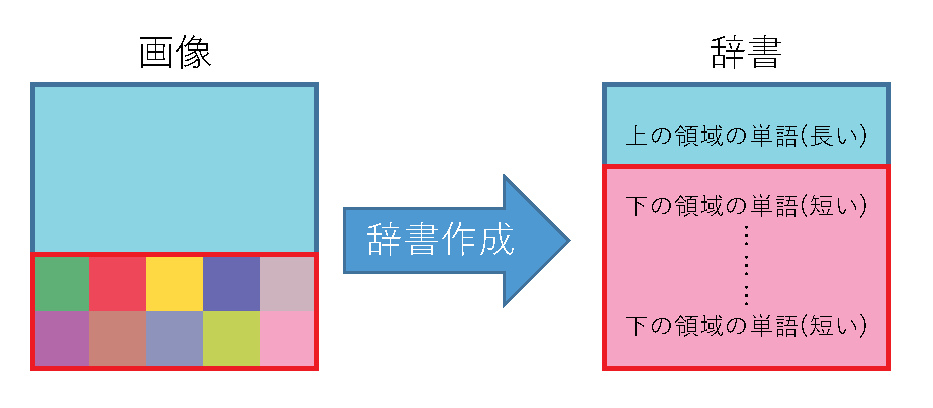
\includegraphics[clip, width=\columnwidth]{image/created_image_1.eps}
\caption{単純な領域と複雑な領域に対する辞書内での単語の割合}
\label{fig:created_image.eps}
\end{center}
\end{figure}
\section{重み付きNMD}
前節で述べた課題に対して,本研究では単語ごとに重みを付けて類似度を計算する
重み付き辞書間距離 WNMD (weigtbed NMD)を提案する.$x,y$間の距離$WNMD(x,y)$は次のように
定義される.
%単語がオブジェクト中で占める長さによらず,類似度計算に与える影響に差がない問題を回避するために,単語ごとに重みをつけることを考える.
%次のような
$$
\frac{G(MS(x) \cup MS(y)) - \min(G(MS(x)) , G(MS(y)))}{\max(G(MS(x)) , G(MS(y)))}
$$
\begin{equation}
G(MS(x)) = \sum_{i=1}^n g(w_i)\times m_i^x
\end{equation}
ここで,$g(w_i)$は単語$w_i$に対する重みである.

% 関数$g$は単語の長さに関して単調増加することが望ましい.
単語に対する重みは,その情報量を表すものが理想だが,正確な情報量は求めることが困難である.
そこで本研究では,単語$w$の重み$g(w)$を,$w$が全て同一文字から構成される場合の最小記述長から定める.

文字列$T=\underbrace{\mbox{aa}\cdots \mbox{a}}_{|w|}$は,$a$が$\sqrt{|w|}$回連続した文字列$A=\underbrace{\mbox{aa}\cdots \mbox{a}}_{\sqrt{|w|}}$を符号語
(モデル)として,$\underbrace{\mbox{AA}\cdots \mbox{A}}_{\sqrt{|w|}}$と表記した時に,
$$記述長=(モデルAの長さ)+(AによるTの符号列長)$$
が最小になる.この時の記述長は$O(\sqrt{|w|})$になることから,$g(|w|)$を式(\ref{eq:weigtbWNMD})とした.ここで,$|w|$は単語$w$の文字数である.
\begin{equation}
\label{eq:weigtbWNMD}
g(w)=\sqrt{|w|}.
\end{equation}

%重みは$log_2(単語の長さ)$とする.
% section nmdの改良_仮_ (end)